% ----- Consignes exo 1 ----- %
\iftoggle{showquestions}{
    \begin{td-exo}[Antigone des asso]\,\\ % 1
        Un groupe de personnes est tel que:
        \begin{enumerate}
            \item Chaque personne est membre d'exactement deux associations,
            \item chaque association comprend exactement trois membres,
            \item deux associations ont toujours exactement un membre en commun.
        \end{enumerate}
        Combien y a-t-il de personnes? D'associations?
    \end{td-exo}
}{}

% ----- Solutions exo 1 ----- %
\begin{td-sol}[]\,\\ % 1
    Il y a exactement 6 personnes et 4 associations avec l'arrangement qui suit:

    \vspace{0.5cm}
    \ffigbox[\FBwidth]{%
\label{Fig:dm1ex1}
}{
    \fbox{
        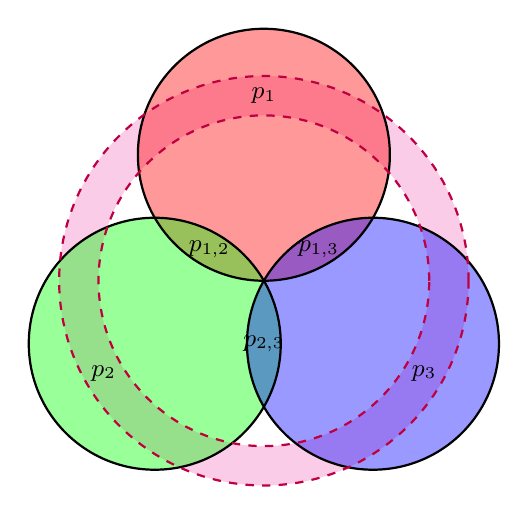
\begin{tikzpicture}[scale=1, every node/.style={circle, draw, fill=blue!20, inner sep=1pt, font=\scriptsize, minimum size=4mm}]
            % centers of the three circles
            \coordinate (A) at (90:1.6cm);
            \coordinate (B) at (210:1.6cm);
            \coordinate (C) at (330:1.6cm);
            \def\r{1.6cm} % radius (adjust as desired)
            
            % Add the circular band/strip
            \def\bandInnerRadius{2.1cm}
            \def\bandOuterRadius{2.6cm}

            % Draw the band with some transparency
            \fill[magenta, fill opacity=0.2] (0,0) circle (\bandOuterRadius);
            \fill[white] (0,0) circle (\bandInnerRadius);

            % draw filled circles with transparency
            \fill[red,   fill opacity=0.4]  (A) circle (\r);
            \fill[green, fill opacity=0.4]  (B) circle (\r);
            \fill[blue,  fill opacity=0.4]  (C) circle (\r);

            % remove (mask out) the triple-intersection area
            \begin{scope}
                \clip (A) circle (\r);
                \clip (B) circle (\r);
                \clip (C) circle (\r);
                % filling a large rectangle inside the triple-clip erases that area
                \fill[white] (-3,-3) rectangle (3,3);
            \end{scope}

            % circle outlines
            \draw[line width=0.8pt] (A) circle (\r);
            \draw[line width=0.8pt] (B) circle (\r);
            \draw[line width=0.8pt] (C) circle (\r);
            
            % Optional: Add outline for the band
            \draw[line width=0.8pt, purple, dashed] (0,0) circle (\bandInnerRadius);
            \draw[line width=0.8pt, purple, dashed] (0,0) circle (\bandOuterRadius);

            % Updated labels - moved to intersections between strip and circles
            \node[circle, draw=none, fill=none, font=\small] at (90:2.35cm) {\(p_1\)}; % Top circle
            \node[circle, draw=none, fill=none, font=\small] at (210:2.35cm) {\(p_2\)}; % Bottom left circle
            \node[circle, draw=none, fill=none, font=\small] at (330:2.35cm) {\(p_3\)}; % Bottom right circle

            % Labels for pairwise intersections (unchanged)
            \node[circle, draw=none, fill=none, font=\small] at (30:0.8cm) {\(p_{1,3}\)}; % A∩C
            \node[circle, draw=none, fill=none, font=\small] at (150:0.8cm) {\(p_{1,2}\)}; % A∩B
            \node[circle, draw=none, fill=none, font=\small] at (270:0.8cm) {\(p_{2,3}\)}; % B∩C
        \end{tikzpicture}
    }
}

    On peut bien vérifier qu'avec les associations
    \begin{itemize}
        \item \(\color{red}A = \{p_1, p_{1,2}, p_{1,3}\}\),
        \item \(\color{green}B = \{p_2, p_{1,2}, p_{2,3}\}\)
        \item \(\color{blue}C = \{p_3, p_{1,3}, p_{2,3}\}\)
        \item \(\color{magenta}D = \{p_1, p_2, p_3\}\)
    \end{itemize}
    on respecte bien les trois contraintes:
    \begin{enumerate}
        \item Chaque personne est membre d'exactement deux associations:
        \begin{itemize}
            \item \(p_1\) est dans \(A\) et \(D\),
            \item \(p_2\) est dans \(B\) et \(D\),
            \item \(p_3\) est dans \(C\) et \(D\),
            \item \(p_{1,2}\) est dans \(A\) et \(B\),
            \item \(p_{1,3}\) est dans \(A\) et \(C\),
            \item \(p_{2,3}\) est dans \(B\) et \(C\).
        \end{itemize}
        \item Chaque association comprend exactement trois membres: 
        \begin{equation*}
            |A| = |B| = |C| = |D| = 3
        \end{equation*}
        \item Deux associations ont toujours exactement un membre en commun:
        \begin{itemize}
            \item \(A\cap B = \{p_{1,2}\}\),
            \item \(A\cap C = \{p_{1,3}\}\),
            \item \(A\cap D = \{p_1\}\),
            \item \(B\cap C = \{p_{2,3}\}\),
            \item \(B\cap D = \{p_2\}\),
            \item \(C\cap D = \{p_3\}\).
        \end{itemize}
    \end{enumerate}
\end{td-sol}


% ----- Consignes exo 2 ----- %
\iftoggle{showquestions}{
    \begin{td-exo}[Bipartis]\,\\ % 2
        Montrer proprement qu'un graphe \(G\) est biparti si et 
        seulement si il ne contient pas de cycle de longueur impaire.

        De plus, donner un algorithme linéaire (en \(O(n+m)\))
        pour décider si un graphe est biparti ou non.
    \end{td-exo}
}{}

% ----- Solutions exo 2 ----- %
\begin{td-sol}[]\,\\ % 2
    Montrons qu'un graphe est biparti si et seulement si il ne contient pas de cycle impair comme sous-graphe.
    \begin{itemize}
        \item Sens direct: Supposons que \(G\) est biparti. Soit \(C\) un cycle de \(G\).
        Par définition d'un graphe biparti, on peut colorier les sommets de \(G\)
        en deux couleurs telles que deux sommets adjacents
        n'aient pas la même couleur. En parcourant le cycle \(C\), on remarque
        que chaque sommet doit avoir une couleur différente du sommet précédent.
        Ainsi, si le cycle \(C\) a une longueur impaire, le premier et le dernier
        sommet du cycle \(C\) seraient de la même couleur, ce qui est impossible
        car ils sont adjacents. Donc \(C\) ne peut pas être de longueur impaire.

        \begin{figure}[H]
	\CenterFloatBoxes{}		% centers the floatrow contents horizontally
	\begin{floatrow}
		% Figure 1
\ffigbox[\FBwidth]{
\caption{\centering Cas cycle pair}\label{Fig:td1ex3c2}
}{
    \fbox{
        \resizebox{!}{3cm}{%
            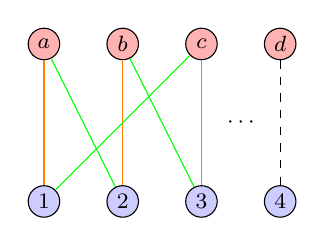
\begin{tikzpicture}[scale=1, every node/.style={circle, draw, fill=blue!20, inner sep=1pt, font=\footnotesize, minimum size=4mm}]
                \node[fill=red!30] (a) at (0, 2) {\(a\)};
                \node[fill=red!30] (b) at (1, 2) {\(b\)};
                \node[fill=red!30] (c) at (2, 2) {\(c\)};
                \node[fill=red!30] (d) at (3, 2) {\(d\)};

                \node (1) at (0, 0) {\(1\)};
                \node (2) at (1, 0) {\(2\)};
                \node (3) at (2, 0) {\(3\)};
                \node (4) at (3, 0) {\(4\)};

                \node[draw=none, fill=none] (dots) at (2.5, 1) {\(\cdots\)};

                \draw[orange] (a) -- (1);
                \draw[orange] (b) -- (2);
                \draw[orange] (c) -- (3);

                \draw[green] (1) -- (c);
                \draw[green] (2) -- (a);
                \draw[green] (3) -- (b);
                
                \draw[dashed] (d) -- (4);
            \end{tikzpicture}
        }
    }
}

		% Figure 1
\ffigbox[\FBwidth]{
\caption{\centering Cas cycle impair}\label{Fig:td1ex3c1}
}{
    \fbox{
        \resizebox{!}{3cm}{%
            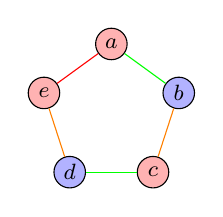
\begin{tikzpicture}[scale=0.45, every node/.style={circle, draw, fill=blue!20, inner sep=1pt, font=\footnotesize, minimum size=4mm}]
                \node[fill=red!30] (A) at (90:2) {\(a\)};
                \node[fill=blue!30] (B) at (18:2) {\(b\)};
                \node[fill=red!30] (C) at (-54:2) {\(c\)};
                \node[fill=blue!30] (D) at (-126:2) {\(d\)};
                \node[fill=red!30] (E) at (162:2) {\(e\)};

                \draw[green] (A) -- (B);
                \draw[orange] (B) -- (C);
                \draw[green] (C) -- (D);
                \draw[orange] (D) -- (E);
                \draw[red] (E) -- (A);
            \end{tikzpicture}
        }
    }
}
	\end{floatrow}
\end{figure}

        \item Sens indirect: Supposons que \(G\) ne contient pas de cycle impair.
        On choisit un sommet racine \(r\) et on effectue un parcours en largeur à partir de \(r\).
        On colorie le sommet \(r\) en rouge. Ensuite, on colorie tous les sommets
        de niveau 1 (voisins de \(r\)) en bleu, tous les sommets de niveau 2 en rouge,
        tous les sommets de niveau 3 en bleu, et ainsi de suite.

        \begin{figure}[H]
	\CenterFloatBoxes{}		% centers the floatrow contents horizontally
	\begin{floatrow}
		% Figure 1
\ffigbox[\FBwidth]{
\caption{\centering Premiere etape du BFS}\label{Fig:td1ex3c3}
}{
    \fbox{
        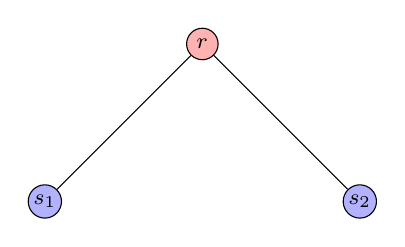
\begin{tikzpicture}[scale=1, every node/.style={circle, draw, fill=blue!20, inner sep=1pt, font=\footnotesize, minimum size=4mm}]
            \node[fill=red!30] (r) at (0, 0) {\(r\)};
            \node[fill=blue!30] (s1) at (-2, -2) {\(s_1\)};
            \node[fill=blue!30] (s2) at (2, -2) {\(s_2\)};

            \draw (r) -- (s1);
            \draw (r) -- (s2);
        \end{tikzpicture}
    }
}

		% Figure 1
\ffigbox[\FBwidth]{
\caption{\centering Deuxieme etape du BFS}\label{Fig:td1ex3c4}
}{
    \fbox{
        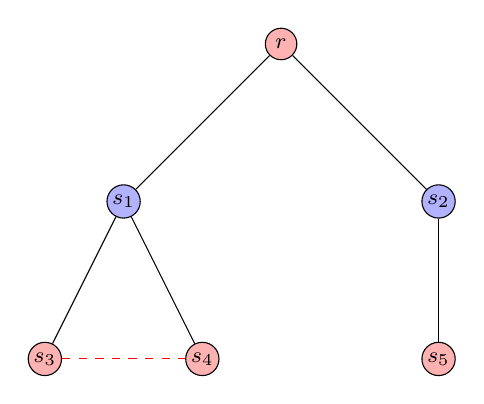
\begin{tikzpicture}[scale=1, every node/.style={circle, draw, fill=blue!20, inner sep=1pt, font=\footnotesize, minimum size=4mm}]
            \node[fill=red!30] (r) at (0, 0) {\(r\)};
            \node[fill=blue!30] (s1) at (-2, -2) {\(s_1\)};
            \node[fill=blue!30] (s2) at (2, -2) {\(s_2\)};

            \node[fill=red!30] (s3) at (-3, -4) {\(s_3\)};
            \node[fill=red!30] (s4) at (-1, -4) {\(s_4\)};
            \node[fill=red!30] (s5) at (2, -4) {\(s_5\)};

            \draw (r) -- (s1);
            \draw (r) -- (s2);

            \draw (s1) -- (s3);
            \draw (s1) -- (s4);
            \draw (s2) -- (s5);

            \draw[red, dashed] (s3) -- (s4);
        \end{tikzpicture}
    }
}
	\end{floatrow}
\end{figure}

        Si il y avait une arête entre deux sommets du même niveau, cela formerait
        un cycle impair avec le chemin passant par leur parent commun \(r_i\). En effet,
        si deux sommets \(u\) et \(v\) sont au même niveau et sont adjacents,
        alors le chemin de \(r_i\) à \(u\), l'arête \((u,v)\), et le chemin de
        \(v\) à \(r_i\) forment un cycle dont la longueur est impaire (car la 
        distance de \(r_i\) à \(u\) et \(v\) est la même, disons \(d\), donc le cycle a une longueur de \(2d + 1\)).
        
        Cependant, par hypothèse, \(G\) ne contient pas de cycle impair.
        Donc, il ne peut pas y avoir d'arêtes entre deux sommets du même niveau.
        Par conséquent, tous les sommets de niveau pair sont colorés en rouge et tous les sommets de niveau impair sont colorés en bleu.
        Ainsi, \(G\) est biparti.

        Un algorithme permettant de décider si un graphe est biparti ou non est donc celui 
        décrit ci-dessus, avec une complexité en \(O(n+m)\) car chaque sommet et chaque arête
        est visité au plus une fois lors du parcours en largeur.
    \end{itemize}
\end{td-sol}



% ----- Consignes exo 3 ----- %
\iftoggle{showquestions}{
    \begin{td-exo}[Graphes sans triangles]\,\\ % 3
        Le but de l'exercice est de montrer que si \(G\) ne contient pas 
        de triangle alors le nombre d'arêtes de \(G\) est au plus
        \(\frac{n^2}{4}\) si \(n\) est pair et au plus \(\frac{n^2-1}{4}\) si \(n\) est impair.
        \begin{enumerate}
            \item On raisonne par récurrence sur \(n\). Soit \(uv\) une arête de \(G\).
            Majorer le nombre d'arêtes entre \(\{u,v\}\) et \(V\setminus\{u,v\}\)
            puis conclure.
            \item Quels sont les graphes sans triangle qui ont pour 
            nombre d'arêtes exactement les bornes proposées?
        \end{enumerate}
    \end{td-exo}
}{}

% ----- Solutions exo 3 ----- %
\begin{td-sol}[]\, % 3
    \begin{enumerate}
        \item On peut commencer par remarquer que comme \(G\) est sans triangles,
        les voisins de \(u\) et \(v\) sont disjoints (en effet si 
        on note \(w\) un voisin commun aux 2 alors \(uvw\) forme un triangle).
        
        Alors, le nombre d'arêtes entre \(\{u,v\}\) et \(V\setminus\{u,v\}\)
        est le nombre d'arêtes entre \(u\) et \(V\setminus\{u,v\}\)
        plus le nombre d'arêtes entre \(v\) et \(V\setminus\{u,v\}\). Soit
        \begin{equation*}
            \deg(u) - 1 + \deg(v) - 1 = \deg(u) + \deg(v) - 2
        \end{equation*}
        où on a enlevé 1 au degré des deux sommets car ils sont adjacents.

        De plus, comme les voisins de \(u\) et \(v\) sont disjoints,
        on a
        \begin{equation*}
            \begin{aligned}
                \deg(u) - 1 + \deg(v) - 1 &\leq n - 2 \\
                \deg(u) + \deg(v) &\leq n
            \end{aligned}
        \end{equation*}

        Pour ce qui est de la récurrence, si \(n=1\), le graphe
        n'a pas d'arêtes et la propriété est vérifiée.
        Si \(n=2\), le graphe peut avoir au plus une arête
        et la propriété est vérifiée. Montrons que si 
        la propriété est vérifiée pour un graphe de taille \(n-2\),
        elle l'est aussi pour un graphe de taille \(n\).

        On peut catégoriser les arêtes de \(G\) en trois groupes différents:
        \begin{itemize}
            \item L'arête \(uv\) que l'on a choisie,
            \item Les arêtes entre \(\{u,v\}\) et \(V\setminus\{u,v\}\),
            \item Les arêtes entre les sommets de \(V\setminus\{u,v\}\) (on 
            notera \(m'\) leur nombre).
        \end{itemize}
        Ce qui nous donne \(m\), le nombre total d'arêtes de \(G\):
        \begin{equation*}
            m = 1 + \underbrace{(\deg(u) + \deg(v) - 2)}_{\text{arêtes entre } \{u,v\} \text{ et } V\setminus\{u,v\}} + m' = \deg(u) + \deg(v) - 1 + m'
        \end{equation*}

        On procède par disjonction de cas:
        \begin{itemize}
            \item Si \(n = 2k\) est pair, alors \(n-2\) est pair. Par hypothèse de récurrence,
            on a
            \begin{equation*}
                m' \leq \frac{{(n-2)}^2}{4}
            \end{equation*}
            En utilisant notre formule précédente, on a
            \begin{equation*}
                \begin{aligned}
                    m
                    &= \deg(u) + \deg(v) - 1 + m' \\
                    &\leq n - 1 + \frac{{(n-2)}^2}{4} \\
                    &\leq 2k - 1 + \frac{{(2k-2)}^2}{4} \\
                    &\leq 2k - 1 + \frac{4k^2 - 8k + 4}{4} \\
                    &\leq 2k - 1 + k^2 - 2k + 1 \\
                    &\leq k^2 \\
                    &\leq {(\frac{n}{2})}^2 \\
                    &\leq \frac{n^2}{4}
                \end{aligned}
            \end{equation*}
            Donc la formule est vérifiée pour \(n\) pair.

            \item Si \(n = 2k + 1\) est impair, alors \(n-2\) est impair. Par hypothèse de récurrence,
            on a
            \begin{equation*}
                m' \leq \frac{{(n-2)}^2-1}{4}
            \end{equation*}
            En utilisant notre formule précédente, on a
            \begin{equation*}
                \begin{aligned}
                    m
                    &= \deg(u) + \deg(v) - 1 + m' \\
                    &\leq n - 1 + \frac{{(n-2)}^2 - 1}{4} \\
                    &\leq 2k + 1 - 1 + \frac{{(2k-1)}^2 - 1}{4} \\
                    &\leq 2k + \frac{4k^2 - 4k + 1 - 1}{4} \\
                    &\leq 2k + k^2 - k \\
                    &\leq k^2 + k \\
                    &\leq {(\frac{n-1}{2})}^2 + \frac{n-1}{2} \\
                    &\leq \frac{n^2 - 2n + 1 + 2n - 2}{4} \\
                    &\leq \frac{n^2 - 1}{4}
                \end{aligned}
            \end{equation*}
            Donc la formule est vérifiée pour \(n\) impair.
        \end{itemize}
        On a donc montré que si \(G\) est un graphe sans triangles
        alors le nombre d'arêtes de \(G\) est au plus
        \(\frac{n^2}{4}\) si \(n\) est pair et 
        au plus \(\frac{n^2-1}{4}\) si \(n\) est impair.

        \item Pour le cas d'égalité, il faut que toutes les inégalités deviennent des égalités:
        \begin{itemize}
            \item \(\deg(u) + \deg(v) = n\) (les voisins de \(u\) et \(v\) partitionnent \(V\setminus\{u,v\}\))
            \item \(G \setminus \{u,v\}\) atteint sa borne maximale (donc est un graphe biparti complet équilibré par l'hypothèse de récurrence)
            \item Tous les sommets d'une partie de \(G \setminus \{u,v\}\) sont connectés à \(u\), et tous les sommets de l'autre partie à \(v\)
        \end{itemize}
        Cela nous donne la structure suivante:

        \vspace{0.5cm}
        \ffigbox[\FBwidth]{%
\caption{\centering Graphe représenté à partir de \(uv\)\\(les %
autre sommets peuvent être reliés à ceux\\ de l'autre %
côté mais pas entre eux)}\label{Fig:dm1ex3q2}
}{
    \fbox{
        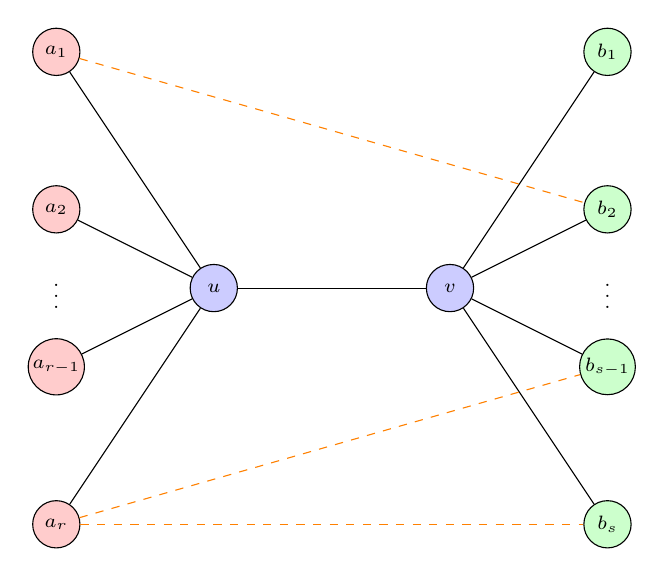
\begin{tikzpicture}[scale=1, every node/.style={circle, draw, fill=blue!20, inner sep=1pt, font=\scriptsize, minimum size=6mm}]
            % les deux sommets initiaux
            \node (u) at (0,0) {\(u\)};
            \node (v) at (3,0) {\(v\)};

            % ceux liés à u
            \node[fill=red!20] (a1) at (-2,3) {\(a_1\)};
            \node[fill=red!20] (a2) at (-2,1) {\(a_2\)};
            \node[fill=red!20] (a3) at (-2,-1) {\(a_{r-1}\)};
            \node[fill=red!20] (a4) at (-2,-3) {\(a_{r}\)};

            % ceux liés à v
            \node[fill=green!20] (b1) at (5,3) {\(b_1\)};
            \node[fill=green!20] (b2) at (5,1) {\(b_2\)};
            \node[fill=green!20] (b3) at (5,-1) {\(b_{s-1}\)};
            \node[fill=green!20] (b4) at (5,-3) {\(b_{s}\)};
            % on relie les sommets
            \foreach \x in {1,2,3,4} {
                \draw (u) -- (a\x);
                \draw (v) -- (b\x);
            }

            % on relie u et v
            \draw (u) -- (v);

            % on relie fictivement d'autres sommets
            \draw[orange, dashed] (a1) -- (b2);
            \draw[orange, dashed] (a4) -- (b3);
            \draw[orange, dashed] (a4) -- (b4);


            % on rajoute les ellipses
            \node[draw=none, fill=none] at (-2,0) {\(\vdots\)};
            \node[draw=none, fill=none] at (5,0) {\(\vdots\)};
        \end{tikzpicture}
    }
}

        En respectant toutes les conditions, on arrive
        bien à un graphe biparti complet où les deux parties
        ont une taille aussi proche que possible:
        \begin{itemize}
            \item La première condition nous impose la partition
            du graphe par \(uv\).
            \item Les autres nous imposent que chaque sommet
            d'une partie soit relié à tous les sommets de l'autre partie
            et pour la maximalité, que les tailles des deux parties
            soient aussi proches que possible (pour maximiser le produit des tailles).

            \item Visuellement cela veut dire qu'il y a une arête 
            entre chaque paire \((a_i,b_j)\) et que \(r\) et \(s\)
            sont distants d'au plus 1.
        \end{itemize}

        Donc la solution est \(G\) un graphe biparti complet
        \(K_{r,s}\) avec \(r+s=n\) et \(|r-s|\leq 1\).
    \end{enumerate}
\end{td-sol}



% ----- Consignes exo 4 ----- %
\iftoggle{showquestions}{
    \begin{td-exo}[Couplage dans les cubiques]\,\\ % 4
        Une arête \(e\) d'un graphe connexe \(G\) est dite séparatrice si 
        \(G - e\) n'est pas connexe.
        \begin{enumerate}
            \item Soit \(G\) un graphe 3-régulier (ou cubique\dots) et \(M\) 
            un couplage parfait de \(G\). Montrer que \(M\) contient 
            toutes les arêtes séparatrices de \(G\).
            \item Donner un exemple de graphe cubique qui n'admet 
            pas de couplage parfait.
            \item Plus généralement, pour tout \(k\geq 2\), proposer un graphe 
            \((2k+1)\)-régulier qui n'admet pas de couplage parfait.
        \end{enumerate}
    \end{td-exo}
}{}

% ----- Solutions exo 4 ----- %
\begin{td-sol}[]\,\\ % 4
    % TODO: completer solution exercice 4
\end{td-sol}



% ----- Consignes exo 5 ----- %
\iftoggle{showquestions}{
    \begin{td-exo}[Pierre, papier, ciseaux]\,\\ % 5
        Lors du tournoi international de Pierre-Papier-Ciseaux,
        vous êtes en charge d'organiser le déroulement des matchs.
        On note \(n\) le nombre de participants. Un match oppose deux 
        participants. Lors du tournoi, chaque participant doit rencontrer 
        chaque autre participant exactement une fois. Le tournoi est 
        découpé en rounds pendant lesquels les match ont lieu, un 
        partipant faisant au plus un match par round. Le but de votre 
        travail est d'organiser les rencontres en minimisant le nombre 
        de rounds.
        \begin{enumerate}
            \item Modéliser le problème (avec un graphe bien choisi).
            \item Résoudre le problème pour \(n=3,4,5,6\).
            \item Donner une réponse pour \(n\) quelconque et 
            justifier votre réponse.
        \end{enumerate}
    \end{td-exo}
}{}

% ----- Solutions exo 5 ----- %
\begin{td-sol}[]\, % 5
    \begin{enumerate}
        \item \,% TODO: completer solution exercice 5
        \item On procède en fonction de \(n\):
        \begin{itemize}
            \item Pour \(n=3\), on note \(p_1,p_2,p_3\) les participants et on a
            \begin{equation*}
                \begin{aligned}
                    R1
                    &\rightarrow (p_1,p_2)\\
                    R2
                    &\rightarrow (p_1,p_3)\\
                    R3
                    &\rightarrow (p_2,p_3)
                \end{aligned}
            \end{equation*}
            Il faut exactement 3 rounds pour que tous les participants s'affrontent.
        
            \item Pour \(n=4\), on a
            \begin{equation*}
                \begin{aligned}
                    R1
                    &\rightarrow (p_1,p_2)\\
                    &\rightarrow (p_3,p_4)\\
                    R2
                    &\rightarrow (p_1,p_3)\\
                    &\rightarrow (p_2,p_4)\\
                    R3
                    &\rightarrow (p_1,p_4)\\
                    &\rightarrow (p_2,p_3)
                \end{aligned}
            \end{equation*}
            Il faut exactement 3 rounds pour résoudre le problème.
        
            \item Pour \(n=5\), on a
            \begin{equation*}
                \begin{aligned}
                    R1
                    &\rightarrow (p_1,p_2)\\
                    &\rightarrow (p_5,p_4)\\
                    R2
                    &\rightarrow (p_1,p_3)\\
                    &\rightarrow (p_5,p_2)\\
                    R3
                    &\rightarrow (p_1,p_4)\\
                    &\rightarrow (p_2,p_3)\\
                    R4
                    &\rightarrow (p_5,p_1)\\
                    &\rightarrow (p_3,p_4)\\
                    R5
                    &\rightarrow (p_2,p_4)\\
                    &\rightarrow (p_5,p_3)\\
                \end{aligned}
            \end{equation*}
            Il faut exactement 5 rounds pour résoudre le problème.
        \end{itemize}
    \end{enumerate}
\end{td-sol}



% ----- Consignes exo 6 ----- %
\iftoggle{showquestions}{
    \begin{td-exo}[Couplage dans les arbres]\,\\ % 6
        Le but de l'exercice est de proposer un algorithme de calcul 
        d'un couplage maximum dans les arbres plus direct que 
        l'algorithme de Egerváry.
        \begin{enumerate}
            \item Soit \(T\) un arbre et \(f\) une feuille de \(T\).
            Montrer que \(T\) admet un couplage maximum qui sature \(f\).
            \item En déduire un algorithme récursif pour le calcul 
            d'un couplage maximum de \(T\).
            \item On propose une implémentation efficace de l'algorithme 
            ci-dessus: on pourra effectuer un parcours en profondeur 
            de \(T\), puis lister les sommets selon l'ordre de \emph{fin}
            obtenu et choisir les arêtes du couplage gloutonnement selon 
            cet ordre. Détailler l'algorithme (on pourra faire appel à 
            un parcours en profondeur), prouver sa validité et calculer 
            sa complexité.
            \item \emph{Question annexe}: montrer qu'un arbre possède au 
            plus un couplage parfait
        \end{enumerate}
    \end{td-exo}
}{}

% ----- Solutions exo 6 ----- %
\begin{td-sol}[]\,\\ % 6
    % TODO: completer solution exercice 6
\end{td-sol}
